\section{Methodology}

\textsc{Date} describes the density-based clustering analysis which is a novel contribution of this work; we also present \textsc{Date} in the context of a larger packet processing system for real AI applications.

\subsection{Point Cloud Creation}
Point clouds are a set of Cartesian coordinates $(x, y, z)$ which represent some points in a three-dimensional space. In computer vision, point clouds may be used as a method for mapping high-dimensional shapes into lower-dimensioned space~\cite{Wang_2019_ICCV}. This latent representation is often used in a temporal sense to express the movement of objects in three-dimensional space. For example, a car may be modeled as a 3D point cloud, and its movement in space described as a series of clouds ${c_0, c_1,...,c_t}$ where $t$ represents a number of time intervals and $c_n$ the point cloud generated at a given time slice. Unlike time-series based approaches which would require traffic flow data, we emulate the work of Quach et al~\cite{Quach2020compression} and treat the point clouds as static, analagous to manifolds in three dimensional space. This captures a geometrical representation of packet data which we use for cluster analysis.

In the \textsc{Date} model, payload data is extracted from the packets and truncated to 1024 bytes. In cases where the payload is shorter than 1024, we add padding to normalize the input size. We convert the byte values $v$ to decimal values $v' \in [0,255]$. A sliding window technique is then used to create three-dimensional points in our feature space. We map each byte to a value in the $(x, y, z)$ coordinate. The coordinates are mapped to a three-dimensional space to form point clouds like Figure~\ref{fig:cloud}. We expect that packets with similar data will thus result in similar point clouds.

For example, the byte string, `0x68', `0x65', `0x6c', `0x6c', `0x6f', would first be transformed to decimal values (104, 101, 108, 108, 111). Then, the sliding window would produce the points corresponding to coordinates
\begin{equation}
\begin{split}
     C =
\{(104, 101, 108), \\ (101, 108, 108), \\ (108, 108, 111)\}.
\end{split}
\end{equation}

\begin{figure} [ht!]
\centering
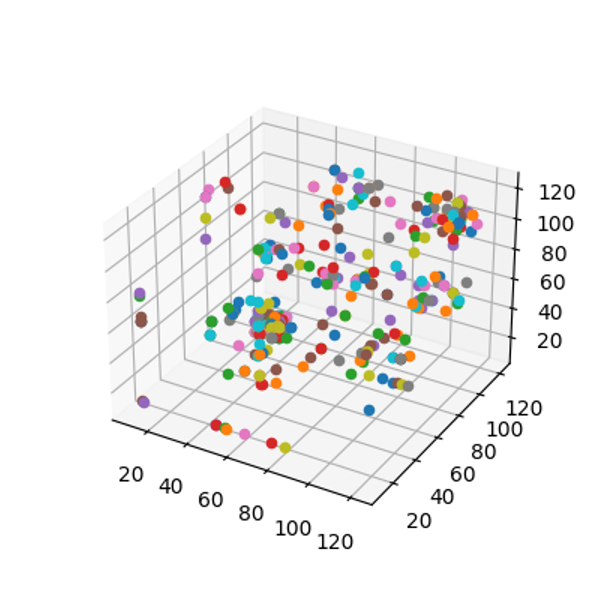
\includegraphics[width=0.6\textwidth]{chapters/6/img/sipcloud.png}
\caption{3D point cloud made out of a Session Initiation Protocol (SIP) packet.}
\label{fig:cloud}
\end{figure}

\subsection{Density-Based Spatial Clustering of Applications With Noise (DBSCAN)}

Density-Based Spatial Clustering of Applications with Noise (DBSCAN) uses three different point classifications (see Figure~\ref{fig:dbscan}): \textit{Core points} represent centers of clusters and points are labeled as such based on the number of neighbors they have compared to their neighbors. \textit{Border points} represent the edges and possess the least number of neighbors but are still within the range of a core point. Noise or \textit{Outlier points} are neither borders nor cores and do not belong to a cluster. The DBSCAN algorithm visits each point and classifies them as such in order to paint a picture of where clusters of data are~\cite{schubert2017dbscan}.

\begin{figure} [ht!]
\centering
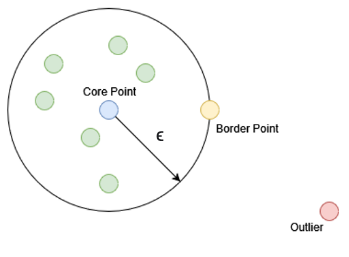
\includegraphics[scale=0.4]{chapters/6/img/dbscan.drawio.png}
\caption{Illustration of types of points in DBSCAN.}
\label{fig:dbscan}
\end{figure}

After the point clouds are created, we process them using the DBSCAN algorithm in order to determine natural clusters that exist in the provided classes in the ground truth. DBSCAN works by grouping points that are close together utilizing a Euclidean distance for measurements. Thresholds exist in the algorithm to specify the minimum number of points needed to create a cluster and the value of the Euclidean distance that determines if points are close enough to make a cluster. We configure two parameters in the algorithm: $\epsilon$ and a minimum number of samples. The $\epsilon$ value is the radius for each circle drawn around each point to query density, and the minimum number of samples is the minimum number of points required to be inside the drawn circle for it to be considered a Core point.

The minimum number of samples must at least be the number of dimensions, and as a heuristic, it is generally twice the dimensions. All tests were performed with the DBSCAN configuration of $\epsilon$ = 7 and \texttt{min\_samples} = 7. Having a baseline of 7 points to make a cluster within a 3D dimensional plane would be forgiving enough to create more clusters in a lower populated point cloud. An $\epsilon$ value of 7 should also allow for a greater number of clusters to be recognized~\cite{rahmah2016determination}.

Tuning DBSCAN has the potential to uncover great performance when it comes to creating recognizable clouds within the 3D space. As stated earlier, two inputs to DBSCAN can be tuned: $\epsilon$ and \texttt{min\_samples}. It is important to have these values set reasonably to see favorable results. As a rule of thumb, the minimum number of samples needed to classify a cluster should be set to at least the number of dimensions. If it is set below this threshold, then singular points or two points that are close together would constitute a cluster, which would not be an accurate way of determining where data is clumped~\cite{mullin2020tuning}.

Similarly, $\epsilon$ needs to be set based on general rules. If the value of $\epsilon$ chosen is too small then more clusters will be created, and more data points will be taken as noise. However, if set too large, then a number of smaller clusters will be more likely to merge into one large cluster. One way that a value of $\epsilon$ can be estimated is by examining the input data and finding the average distance between each point and its k nearest neighbors. Because each packet is highly variable, choosing an exact value for $\epsilon$ is a difficult problem. An estimation of $\epsilon$ must be taken from a conglomeration of the packet's $k$-nearest neighbors data where $k$ is the value of \texttt{min\_samples} chosen. As shown in the figure above, the point of each line with the greatest curvature is considered the ideal value for $\epsilon$. A line has been illustrated in Figure~\ref{fig:kneighborsgraph} where an estimated average is made for every sample. The variation in an ideal $\epsilon$ value could be a major factor in why some packets are recognizable in their cloud state and others are not~\cite{rahmah2016determination}.

We extract the following features as the feature vector for classification from the DBSCAN results:
\begin{itemize}
    \item clusterCount = number of clusters
    \item averageClusterSize = average cluster size
    \item standardDeviation = standard deviation
    \item noisePercent = percent of cloud containing noise
\end{itemize}

\begin{figure} [ht!]
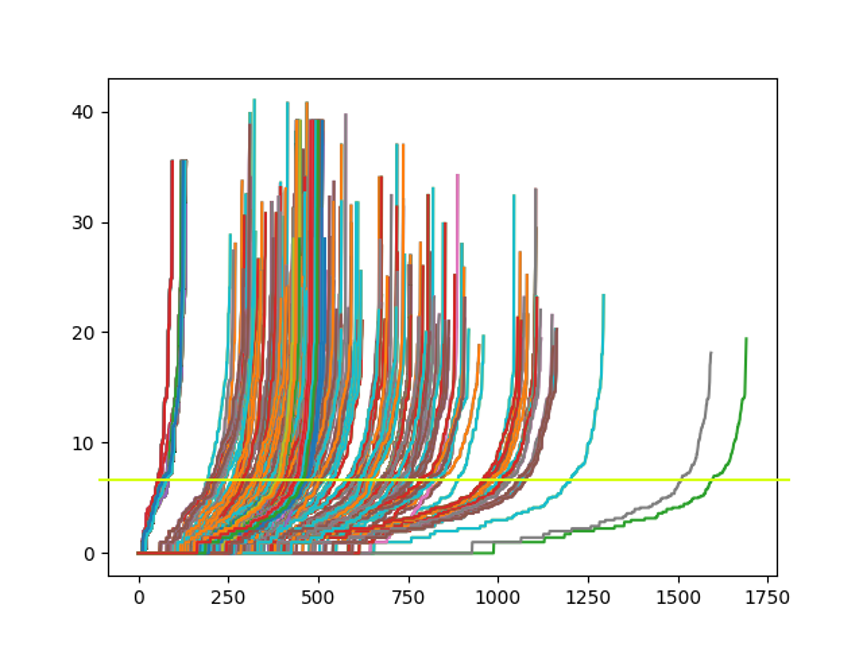
\includegraphics[width=\linewidth]{chapters/6/img/kmembersgraph.png}
\caption{K-nearest neighbors graph generated for packets in the dataset using a \texttt{min\_samples} = 6.}
\label{fig:kneighborsgraph}
\end{figure}

\subsection{Packet Classification}
For deep learning, we feed the extracted cluster features forward into a two-layer multilayer perceptron unit (MLP) with a final softmax layer for classification. We use binary cross entropy as the loss function.
